\documentclass{report}

\usepackage[T1]{fontenc}
\usepackage[american]{babel}
\usepackage{hyperref}
\usepackage{geometry}
\usepackage{graphicx}
\geometry{hmargin=2.5cm,vmargin=1.5cm}

\begin{document}

\title{MicronetToNMEA}

\chapter {Introduction}

\section{What is MicronetToNMEA}

MicronetToNMEA is a Teensy/Arduino based project aimed at building a cheap NMEA/Micronet bridge. The initial purpose of this project was to understand Micronet wireless protocol and to be able to record wind and speed data on a PC. The understanding of the protocol went so well that MicronetToNMEA is now doing a lot more than that. It can:

\begin{itemize}
\item Send NMEA stream to your PC/Tablet with data on depth, water speed, wind, magnetic heading, GNSS positionning, speed, time, etc.
\item Send Heading data from the navigation compass to your Micronet's displays (HDG).
\item Send GNSS data to your Micronet displays (LAT, LON, TIME, DATE, COG, SOG).
\item Send navigation data from OpenCPN or qtVlm to your Micronet displays (BTW, DTW, XTE, ETA).
\end{itemize}

\section{What is NOT MicronetToNMEA}

MicronetToNMEA is not waterproof and more generally not reliable. All electronics used in this project are made for hobbyist and are all but robust. In the brutal, wet and salty environment of a boat, it will likely fail quickly. So be careful that MicronetToNMEA shouldn’t be used as primary navigation tool. Also note that Micronet wireless protocol has been reverse engineered and that many of its aspects are not yet properly understood. Worse, some understandings we think to be correct might very well be false in some circumstances. If you need state of the art and reliable navigation devices, just go to your nearest Raymarine/TackTick reseller.

\section{Contributors}

\begin{itemize}
\item  Ronan Demoment : Main author
\item Dietmar Warning : LSM303 drivers \& Bugfixes
\item Contributors of YBW forum's Micronet thread : \href{https://forums.ybw.com/index.php?threads/raymarines-micronet.539500/}{Micronet Thread}
\end{itemize}

\chapter{Needed hardware and software}

\section{Required hardware}

To work properly, MicronetToNMEA needs at least a Teensy 3.5 board and a CC1101 based breakout board.

\subsection{Teensy 3.5}
In theory, you can port MicronetToNMEA SW to any 32bit Arduino compatible board. Practically, this might be a different story. Several people got into troubles trying to use ESP32 boards. While this is technically feasible, Arduino's library implementation between Teensy \& Esp32 board can be slightly different in some sensitive areas like interrupt handling, making porting complex.
Teensy boards can be ordered here : \url{https://www.pjrc.com/teensy/}

\subsection{CC1101 board}

These boards are very cheap but the quality of the design and components is often average. So do not expect to have the same distance performance than an original TackTick device. Be careful when ordering this board since it is designed for a specific range of frequencies (filter and antenna) even if the board is announced to support 434 \& 868 (the IC can, but the board cannot). MicronetToNMEA needs a board designed for 868MHz usage. Ordering the wrong board would dramatically reduce operating distance between MicronetToNMEA and TackTick devices. Example of suitable board:
\href{https://www.amazon.fr/laqiya-cc1101-868-MHz-Transmission-Antenne-Transceiver/dp/B075PFQ57G}{868MHz CC1101}

\section{Optional hardware}

You can add optional HW to MicronetToNMEA to enhance its capabilities.

\subsection{NMEA0183 GNSS}

If you want to connect a GNSS/GPS to MicronetToNMEA, there is only one important point : it must output its data to the NMEA0183 format. An example of cheap GNSS which fits the need is the UBLOX NEO-M8N. The NEO-M8N can directly output NMEA stream to its serial output. Be careful however to ensure that the model youorder is not counterfeit and really has flash memory to save its configuration. Avoid too cheap offers from unknown HW sources.

\subsection{LSM303DLH or LSM303DLHC navigation compass breakout board}

Connected to Teensy I2C bus, this IC will allow getting magnetic heading. MicronetToNMEA automatically detect the presence and type of LSM303DLH(c) on its I2C bus.

\subsection{HC-06 Bluetooth transceiver}

You can connect HC-06 device to MicronetToNMEA serial NMEA output to easily get a wireless connection to a PC/Tablet. Note that MicronetToNMEA does not configure HC-06 link, it is up to you to configure HC-06 before connecting it.

\section{Required software}

\subsection{Arduino IDE (required)}
Arduino IDE provides gcc-arm compiler and all libraries necessary for MicronetToNMEA. This is the first software you must install.

\subsection{Teensyduino (required)}

Teensyduino is an extension to Arduino IDE which add full support to all Teensy’s board, including Teensy 3.5. It must be installed on top of Arduino IDE to enable compilation for Teensy 3.5.

\section{Optional software}

\subsection{Sloeber (optional)}

If you plan to do more than just compile MicronetToNMEA’s code, you probably need a more serious IDE. Sloeber is an Arduino compatible version of Eclipse. It provides many useful features, which will highly improve your productivity. It requires Arduino IDE and Teensyduino to be already installed.

\chapter{Compilation}

\section{With Arduino IDE}

Here are the steps to compile MicronetToNMEA with Arduino IDE:

\begin{itemize}
\item Get the source code from MicronetToNMEA repository (\url{https://github.com/Rodemfr/MicronetToNMEA})
\item Double-click on MicronetToNMEA.ino. This should open Arduino IDE.
\item In Arduino IDE, select Teensy 3.5 target HW with menu “Tools->Board->Teensyduino->Teensy3.5”
\item Go to menu “Tools->Manage Libraries...” and install the following libraries : SmartRC-CC1101-Driver-Lib and TeensyTimerTool
\item Click on “Verify” button in the button bar, this should compile the project without error.
\item Connect your Teensy 3.5 board onto USB port of your PC and Click “Upload” button to upload MicronetToNMEA binary into Teensy flash memory
\end{itemize}

\section{With Sloeber}

Here are the steps to compile MicronetToNMEA with Sloeber IDE:

\begin{itemize}
\item Before trying to compile with sloeber, you must have successfully compiled with Arduino IDE
\item Start Sloeber and create your Workspace as requested Select menu “File->New->Arduino Sketch"
\item In Sloeber, select menu Arduino->Preferences
\item Add Arduino's library and hardware path in the path lists
\item Exit the panel by clicking "Apply and Close"
\item Select menu File->New-Arduino Sketch
\item Name your project "MicronetToNMEA"
\item Don't use default project location and set the location to your git cloned repository of MicronetToNMEA
\item Click "Next"
\item Select Teensy's platform folder
in the corresponding drop down menu
\item Select "Teensy 3.5" board
\item Select "Faster" optimization
\item Select "Serial" USB Type
\item Select 120MHz CPU Speed
\item Click "Next"
\item Select "No file" as code
\end{itemize}

Your project should be compiling now.

Note that Sloeber can be somewhat picky with toolchain ort library paths. So don’t be surprised if you have to handle additional issues to compile with it. The effort is worth, code productivity with Eclipse is way beyond Arduino IDE.

\section{Compile time configuration}

By default, MicronetToNMEA is configured for a specific HW layout. This means that it is configured to be connected through specific SPI, I2C or GPIO pins to various boards. This configuration can be changed to some extent to adapt your own needs. The file bearing this configuration is “BoardConfig.h”.Note that no coherency check are made in the software. It is your responsibility to provide a reachable configuration (i.e. not to connect SPI wires to non SPI capable pins). Table {\ref{table:configswitches}} lists all available switches and their meaning.

\begin{table}[h]
	\begin{tabular}{|l|p{12cm}|}
		\hline
		NAVCOMPASS\_I2C & Sets the I2C bus to which the navigation compass (i.e. LSM303DLH(C)) is connected. Defined as per “Wiring” library definition (Wire0, Wire1, etc.)\\
		\hline
		RF\_SPI\_BUS & Defines SPI controller connected to RF IC (SPI, SPI1, SPI2)\\
		\hline
		RF\_CS0\_PIN & Defines SPI Chip Select line connected to RF IC\\
		\hline
		RF\_MOSI\_PIN & Defines MOSI pin of SPI bus connected to RF IC\\
		\hline
		RF\_MISO\_PIN & Defines MISO pin of SPI bus connected to RF IC\\
		\hline
		RF\_SCK\_PIN & Defines SCK pin of SPI bus connected to RF IC\\
		\hline
		RF\_GDO0\_PIN & Defines GDO0 pin of SPI bus connected to RF IC\\
		\hline
		LED\_PIN & Defines the pin driving the LED, which is used for error signaling\\
		\hline
		GNSS\_SERIAL & Defines on which serial port is connected the NMEA GNSS (Serial, Serial1, Serial2, etc.)\\
		\hline
		GNSS\_BAUDRATE & Defines on which serial port is connected the NMEA GNSS\\
		\hline
		GNSS\_CALLBACK & Defines the name of the callback function called when new bytes arrive on the
		configured serial port\\
		\hline
		GNSS\_RX\_PIN & Defines serial RX pin connected NMEA GNSS TX pin\\
		\hline
		GNSS\_TX\_PIN & Defines serial TX pin connected NMEA GNSS RX pin\\
		\hline
		USB\_SERIAL & Defines which serial port is connected to USB serial converter\\
		\hline
		USB\_BAUDRATE & Defines baud rate of USB serial converter\\
		\hline
\end{tabular}
	\caption{Configuration switches in BoardConfig.h}
\label{table:configswitches}
\end{table}

\chapter{Installation}

Teensy board must be connected to other boards with the same scheme than you have defined in “BoardConfig.h”. No check is made by MicronetToNMEA software to verify that your configuration is matching your actual connections. You must carefully verify that you properly connected the various devices since a wrong connections can possibly damage your hardware, especially with respect to power supply connections which are mixing 3.3 \& 5V levels.

\section{Power supply}

The first and most important connection to realize is the power supply. You have two options there, you can either :

\begin{itemize}
	\item Power the system via USB
	\item Power the system using external DC power source
\end{itemize}

\subsection{Power via USB}

This is the most straightforward way to power the system : just plug an USB cable in the Teensy connector and it will be powered by the connected PC. Teensy board is equipped with a voltage regulator which provides 3.3V. This 3.3V voltage can be used to power other boards of the system.
Be careful that USB 2.0 limits 5V output current to 500mA, but you should be even more careful since Teensy's regulator recommends not to exceed 250mA for 3.3V. So you must take care that your system does not exceed these limits.
As an example, table \ref{table:boardconsumption} shows maximum current values for various boards.

\begin{table}[h]
	\begin{tabular}{|l|c|c|l|}
		\hline
		Board & Voltage source & Max current & Comment \\
		\hline
		Teensy 3.5 & 3.3V & 50mA & CPU ruuning at 120MHz\\
		CC1101 & 3.3V & 40mA & RF at 868MHz\\
		NEO M8N GNSS & 5V & 45mA & M8N is 3.3V but the board is 5V\\
		LSM303DLH(C) & 3.3V & 10mA & Unspecified in datasheet, value assumed\\
		HC06 Bluetooth transceiver & 3.3V & 40mA & Peak during pairing\\
		\hline
	\end{tabular}
	\caption{Current consumption of typical boards}
	\label{table:boardconsumption}
\end{table}
USB powering is especially useful when you plan to output NMEA through USB-serial. In this case, the connected PC/Tablet will provide power to the system and when MicronetToNMEA is not needed anymore, it will be automatically powered-off when you unplug the cable.

\subsection{Power with an external DC source}
While USB powering is easy to setup, it not a common source of power in a boat. It is more usual to get two wires with an unstable battery voltage between 11V and 15V. In that case, you will need a voltage regulator or a DC-DC converter which will be used to produce a stable 5V for the system. This 5V source can then be connected to the Vin pin of Teensy 3.5. The on-board regulator will then produce 3.3V from this input.
\linebreak
When Vin pin is connected to an external source of power, you must not connect an USB cable to avoid short circuit between Vin and Vusb which are connected together on Teensy by default. The Vin pin can handle voltages from 3.6 to 6V but it is strongly recommended to use 5V here. This way, if you accidentally connect a USB cable while powering Vin, there will be no short circuit.

\begin{figure}
\centering
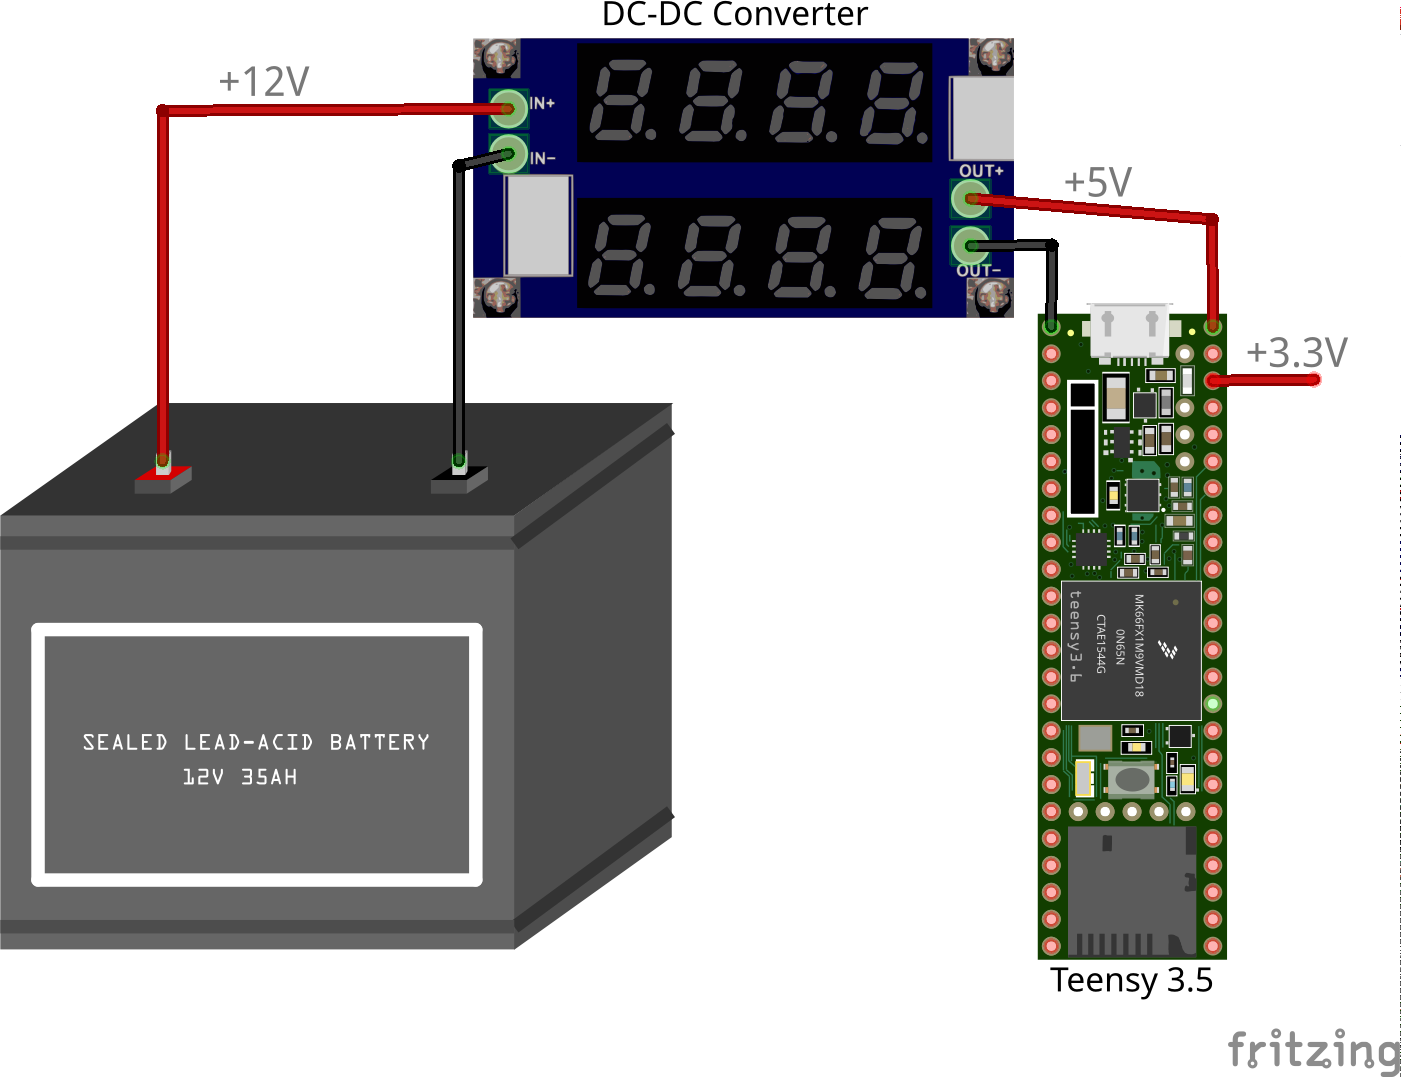
\includegraphics{MicronetToNMEA_DC_Power.png}
	\caption{Powering Teensy with a DC-DC converter}
\label{figure:dcpower}
\end{figure}

\section{Connecting CC1101}

\begin{figure}[h]
	\centering
	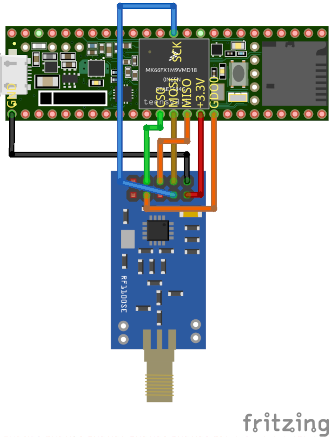
\includegraphics{MicronetToNMEA_CC1101.png}
	\caption{Connecting Teensy to CC1101}
	\label{figure:cc1101}
\end{figure}

\begin{itemize}
\item How to connect
\item Using console
\item Configuring GNSS
\item Configuring HC-06 Bluetooth HW
\end{itemize}

\chapter{Usage}

\begin{itemize}
\item Scanning for Micronet networks
\item Attaching MicronetToNMEA to your existing Micronet networks
\item Calibrating RF frequency
\item Calibrating navigation compass
\item Starting NMEA conversion
\end{itemize}

\chapter{NMEA}

\begin{itemize}
\item Supported sentences (IN and OUT)
\end{itemize}

\chapter{Future}

\begin{itemize}
\item Power consumption
\end{itemize}

\end{document}